% Created by tikzDevice version 0.12.6 on 2024-09-16 10:33:17
% !TEX encoding = UTF-8 Unicode
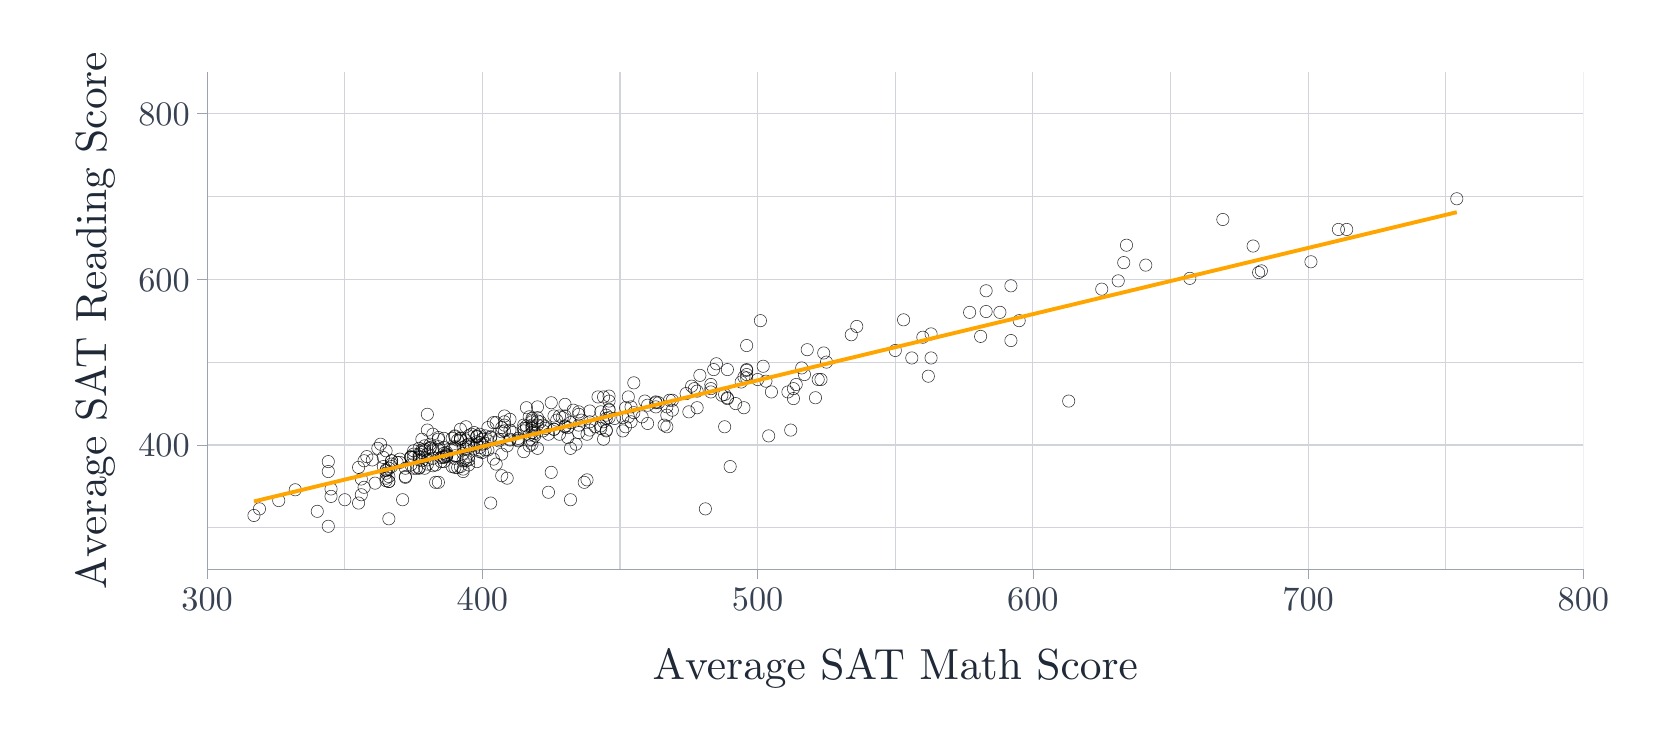
\begin{tikzpicture}[x=1pt,y=1pt]
\definecolor{fillColor}{RGB}{255,255,255}
\path[use as bounding box,fill=fillColor] (0,0) rectangle (578.16,252.94);
\begin{scope}
\path[clip] (  0.00,  0.00) rectangle (578.16,252.94);
\definecolor{drawColor}{RGB}{255,255,255}

\path[draw=drawColor,line width= 0.7pt,line join=round,line cap=round,fill=fillColor] (  0.00,  0.00) rectangle (578.16,252.94);
\end{scope}
\begin{scope}
\path[clip] ( 64.86, 57.20) rectangle (562.16,236.94);
\definecolor{drawColor}{RGB}{255,255,255}
\definecolor{fillColor}{RGB}{255,255,255}

\path[draw=drawColor,line width= 0.7pt,line join=round,line cap=round,fill=fillColor] ( 64.86, 57.20) rectangle (562.16,236.94);
\definecolor{drawColor}{RGB}{209,213,219}

\path[draw=drawColor,line width= 0.4pt,line join=round] ( 64.86, 72.17) --
	(562.16, 72.17);

\path[draw=drawColor,line width= 0.4pt,line join=round] ( 64.86,132.09) --
	(562.16,132.09);

\path[draw=drawColor,line width= 0.4pt,line join=round] ( 64.86,192.01) --
	(562.16,192.01);

\path[draw=drawColor,line width= 0.4pt,line join=round] (114.59, 57.20) --
	(114.59,236.94);

\path[draw=drawColor,line width= 0.4pt,line join=round] (214.05, 57.20) --
	(214.05,236.94);

\path[draw=drawColor,line width= 0.4pt,line join=round] (313.51, 57.20) --
	(313.51,236.94);

\path[draw=drawColor,line width= 0.4pt,line join=round] (412.97, 57.20) --
	(412.97,236.94);

\path[draw=drawColor,line width= 0.4pt,line join=round] (512.43, 57.20) --
	(512.43,236.94);

\path[draw=drawColor,line width= 0.4pt,line join=round] ( 64.86,102.13) --
	(562.16,102.13);

\path[draw=drawColor,line width= 0.4pt,line join=round] ( 64.86,162.05) --
	(562.16,162.05);

\path[draw=drawColor,line width= 0.4pt,line join=round] ( 64.86,221.97) --
	(562.16,221.97);

\path[draw=drawColor,line width= 0.4pt,line join=round] ( 64.86, 57.20) --
	( 64.86,236.94);

\path[draw=drawColor,line width= 0.4pt,line join=round] (164.32, 57.20) --
	(164.32,236.94);

\path[draw=drawColor,line width= 0.4pt,line join=round] (263.78, 57.20) --
	(263.78,236.94);

\path[draw=drawColor,line width= 0.4pt,line join=round] (363.24, 57.20) --
	(363.24,236.94);

\path[draw=drawColor,line width= 0.4pt,line join=round] (462.70, 57.20) --
	(462.70,236.94);

\path[draw=drawColor,line width= 0.4pt,line join=round] (562.16, 57.20) --
	(562.16,236.94);
\definecolor{drawColor}{RGB}{0,0,0}

\path[draw=drawColor,draw opacity=0.80,line width= 0.2pt,line join=round,line cap=round] (419.93,162.35) circle (  2.22);

\path[draw=drawColor,draw opacity=0.80,line width= 0.2pt,line join=round,line cap=round] (159.35,105.43) circle (  2.22);

\path[draw=drawColor,draw opacity=0.80,line width= 0.2pt,line join=round,line cap=round] (182.23,110.52) circle (  2.22);

\path[draw=drawColor,draw opacity=0.80,line width= 0.2pt,line join=round,line cap=round] (376.17,118.01) circle (  2.22);

\path[draw=drawColor,draw opacity=0.80,line width= 0.2pt,line join=round,line cap=round] (174.27,103.93) circle (  2.22);

\path[draw=drawColor,draw opacity=0.80,line width= 0.2pt,line join=round,line cap=round] (397.06,174.33) circle (  2.22);

\path[draw=drawColor,draw opacity=0.80,line width= 0.2pt,line join=round,line cap=round] (153.38,100.63) circle (  2.22);

\path[draw=drawColor,draw opacity=0.80,line width= 0.2pt,line join=round,line cap=round] (202.12,106.03) circle (  2.22);

\path[draw=drawColor,draw opacity=0.80,line width= 0.2pt,line join=round,line cap=round] (201.12, 88.65) circle (  2.22);

\path[draw=drawColor,draw opacity=0.80,line width= 0.2pt,line join=round,line cap=round] (145.43,100.93) circle (  2.22);

\path[draw=drawColor,draw opacity=0.80,line width= 0.2pt,line join=round,line cap=round] (194.16,112.62) circle (  2.22);

\path[draw=drawColor,draw opacity=0.80,line width= 0.2pt,line join=round,line cap=round] (216.04,115.61) circle (  2.22);

\path[draw=drawColor,draw opacity=0.80,line width= 0.2pt,line join=round,line cap=round] (210.07,112.02) circle (  2.22);

\path[draw=drawColor,draw opacity=0.80,line width= 0.2pt,line join=round,line cap=round] (167.31, 81.16) circle (  2.22);

\path[draw=drawColor,draw opacity=0.80,line width= 0.2pt,line join=round,line cap=round] (264.78,147.07) circle (  2.22);

\path[draw=drawColor,draw opacity=0.80,line width= 0.2pt,line join=round,line cap=round] (210.07,119.81) circle (  2.22);

\path[draw=drawColor,draw opacity=0.80,line width= 0.2pt,line join=round,line cap=round] (210.07,118.01) circle (  2.22);

\path[draw=drawColor,draw opacity=0.80,line width= 0.2pt,line join=round,line cap=round] (175.26,106.63) circle (  2.22);

\path[draw=drawColor,draw opacity=0.80,line width= 0.2pt,line join=round,line cap=round] (340.37,150.07) circle (  2.22);

\path[draw=drawColor,draw opacity=0.80,line width= 0.2pt,line join=round,line cap=round] (182.23,108.12) circle (  2.22);

\path[draw=drawColor,draw opacity=0.80,line width= 0.2pt,line join=round,line cap=round] (232.95,114.72) circle (  2.22);

\path[draw=drawColor,draw opacity=0.80,line width= 0.2pt,line join=round,line cap=round] (154.38,100.93) circle (  2.22);

\path[draw=drawColor,draw opacity=0.80,line width= 0.2pt,line join=round,line cap=round] (218.03,110.52) circle (  2.22);

\path[draw=drawColor,draw opacity=0.80,line width= 0.2pt,line join=round,line cap=round] (355.29,139.88) circle (  2.22);

\path[draw=drawColor,draw opacity=0.80,line width= 0.2pt,line join=round,line cap=round] (297.60,141.98) circle (  2.22);

\path[draw=drawColor,draw opacity=0.80,line width= 0.2pt,line join=round,line cap=round] (285.66,125.80) circle (  2.22);

\path[draw=drawColor,draw opacity=0.80,line width= 0.2pt,line join=round,line cap=round] (358.27,147.07) circle (  2.22);

\path[draw=drawColor,draw opacity=0.80,line width= 0.2pt,line join=round,line cap=round] (142.44,104.23) circle (  2.22);

\path[draw=drawColor,draw opacity=0.80,line width= 0.2pt,line join=round,line cap=round] (174.27,104.23) circle (  2.22);

\path[draw=drawColor,draw opacity=0.80,line width= 0.2pt,line join=round,line cap=round] (150.40, 97.94) circle (  2.22);

\path[draw=drawColor,draw opacity=0.80,line width= 0.2pt,line join=round,line cap=round] (197.15,114.72) circle (  2.22);

\path[draw=drawColor,draw opacity=0.80,line width= 0.2pt,line join=round,line cap=round] (323.46,141.08) circle (  2.22);

\path[draw=drawColor,draw opacity=0.80,line width= 0.2pt,line join=round,line cap=round] (203.11,107.53) circle (  2.22);

\path[draw=drawColor,draw opacity=0.80,line width= 0.2pt,line join=round,line cap=round] (281.69,136.58) circle (  2.22);

\path[draw=drawColor,draw opacity=0.80,line width= 0.2pt,line join=round,line cap=round] (114.59, 82.36) circle (  2.22);

\path[draw=drawColor,draw opacity=0.80,line width= 0.2pt,line join=round,line cap=round] (139.46, 97.64) circle (  2.22);

\path[draw=drawColor,draw opacity=0.80,line width= 0.2pt,line join=round,line cap=round] (159.35, 97.94) circle (  2.22);

\path[draw=drawColor,draw opacity=0.80,line width= 0.2pt,line join=round,line cap=round] (130.51, 88.95) circle (  2.22);

\path[draw=drawColor,draw opacity=0.80,line width= 0.2pt,line join=round,line cap=round] (215.05,112.02) circle (  2.22);

\path[draw=drawColor,draw opacity=0.80,line width= 0.2pt,line join=round,line cap=round] (209.08,107.23) circle (  2.22);

\path[draw=drawColor,draw opacity=0.80,line width= 0.2pt,line join=round,line cap=round] (232.95,118.31) circle (  2.22);

\path[draw=drawColor,draw opacity=0.80,line width= 0.2pt,line join=round,line cap=round] (219.03,124.60) circle (  2.22);

\path[draw=drawColor,draw opacity=0.80,line width= 0.2pt,line join=round,line cap=round] (173.27, 90.15) circle (  2.22);

\path[draw=drawColor,draw opacity=0.80,line width= 0.2pt,line join=round,line cap=round] (209.08,111.72) circle (  2.22);

\path[draw=drawColor,draw opacity=0.80,line width= 0.2pt,line join=round,line cap=round] (192.17,112.62) circle (  2.22);

\path[draw=drawColor,draw opacity=0.80,line width= 0.2pt,line join=round,line cap=round] (404.02,167.14) circle (  2.22);

\path[draw=drawColor,draw opacity=0.80,line width= 0.2pt,line join=round,line cap=round] (139.46, 98.84) circle (  2.22);

\path[draw=drawColor,draw opacity=0.80,line width= 0.2pt,line join=round,line cap=round] (156.37,107.82) circle (  2.22);

\path[draw=drawColor,draw opacity=0.80,line width= 0.2pt,line join=round,line cap=round] (346.33,157.86) circle (  2.22);

\path[draw=drawColor,draw opacity=0.80,line width= 0.2pt,line join=round,line cap=round] (355.29,159.65) circle (  2.22);

\path[draw=drawColor,draw opacity=0.80,line width= 0.2pt,line join=round,line cap=round] (185.21,110.52) circle (  2.22);

\path[draw=drawColor,draw opacity=0.80,line width= 0.2pt,line join=round,line cap=round] (344.34,141.38) circle (  2.22);

\path[draw=drawColor,draw opacity=0.80,line width= 0.2pt,line join=round,line cap=round] (179.24,107.23) circle (  2.22);

\path[draw=drawColor,draw opacity=0.80,line width= 0.2pt,line join=round,line cap=round] (157.36, 93.44) circle (  2.22);

\path[draw=drawColor,draw opacity=0.80,line width= 0.2pt,line join=round,line cap=round] (252.84,129.39) circle (  2.22);

\path[draw=drawColor,draw opacity=0.80,line width= 0.2pt,line join=round,line cap=round] (170.29,104.23) circle (  2.22);

\path[draw=drawColor,draw opacity=0.80,line width= 0.2pt,line join=round,line cap=round] (145.43,102.43) circle (  2.22);

\path[draw=drawColor,draw opacity=0.80,line width= 0.2pt,line join=round,line cap=round] (154.38, 97.34) circle (  2.22);

\path[draw=drawColor,draw opacity=0.80,line width= 0.2pt,line join=round,line cap=round] (346.33,150.37) circle (  2.22);

\path[draw=drawColor,draw opacity=0.80,line width= 0.2pt,line join=round,line cap=round] (121.56, 86.85) circle (  2.22);

\path[draw=drawColor,draw opacity=0.80,line width= 0.2pt,line join=round,line cap=round] (143.44,101.83) circle (  2.22);

\path[draw=drawColor,draw opacity=0.80,line width= 0.2pt,line join=round,line cap=round] (149.40, 96.14) circle (  2.22);

\path[draw=drawColor,draw opacity=0.80,line width= 0.2pt,line join=round,line cap=round] (246.87,122.50) circle (  2.22);

\path[draw=drawColor,draw opacity=0.80,line width= 0.2pt,line join=round,line cap=round] (193.17,112.02) circle (  2.22);

\path[draw=drawColor,draw opacity=0.80,line width= 0.2pt,line join=round,line cap=round] (241.90,121.61) circle (  2.22);

\path[draw=drawColor,draw opacity=0.80,line width= 0.2pt,line join=round,line cap=round] (319.48,133.59) circle (  2.22);

\path[draw=drawColor,draw opacity=0.80,line width= 0.2pt,line join=round,line cap=round] (180.24,115.61) circle (  2.22);

\path[draw=drawColor,draw opacity=0.80,line width= 0.2pt,line join=round,line cap=round] (166.31,100.34) circle (  2.22);

\path[draw=drawColor,draw opacity=0.80,line width= 0.2pt,line join=round,line cap=round] (445.79,165.05) circle (  2.22);

\path[draw=drawColor,draw opacity=0.80,line width= 0.2pt,line join=round,line cap=round] (223.00,118.01) circle (  2.22);

\path[draw=drawColor,draw opacity=0.80,line width= 0.2pt,line join=round,line cap=round] (147.42, 88.65) circle (  2.22);

\path[draw=drawColor,draw opacity=0.80,line width= 0.2pt,line join=round,line cap=round] (151.39, 98.84) circle (  2.22);

\path[draw=drawColor,draw opacity=0.80,line width= 0.2pt,line join=round,line cap=round] (207.09,109.02) circle (  2.22);

\path[draw=drawColor,draw opacity=0.80,line width= 0.2pt,line join=round,line cap=round] (108.63, 92.55) circle (  2.22);

\path[draw=drawColor,draw opacity=0.80,line width= 0.2pt,line join=round,line cap=round] (189.19,117.41) circle (  2.22);

\path[draw=drawColor,draw opacity=0.80,line width= 0.2pt,line join=round,line cap=round] (259.80,138.08) circle (  2.22);

\path[draw=drawColor,draw opacity=0.80,line width= 0.2pt,line join=round,line cap=round] (182.23,108.72) circle (  2.22);

\path[draw=drawColor,draw opacity=0.80,line width= 0.2pt,line join=round,line cap=round] (182.23,106.63) circle (  2.22);

\path[draw=drawColor,draw opacity=0.80,line width= 0.2pt,line join=round,line cap=round] (226.98,117.71) circle (  2.22);

\path[draw=drawColor,draw opacity=0.80,line width= 0.2pt,line join=round,line cap=round] (142.44, 96.44) circle (  2.22);

\path[draw=drawColor,draw opacity=0.80,line width= 0.2pt,line join=round,line cap=round] (131.50, 95.24) circle (  2.22);

\path[draw=drawColor,draw opacity=0.80,line width= 0.2pt,line join=round,line cap=round] (165.32,100.34) circle (  2.22);

\path[draw=drawColor,draw opacity=0.80,line width= 0.2pt,line join=round,line cap=round] (258.81,115.61) circle (  2.22);

\path[draw=drawColor,draw opacity=0.80,line width= 0.2pt,line join=round,line cap=round] (138.46, 97.64) circle (  2.22);

\path[draw=drawColor,draw opacity=0.80,line width= 0.2pt,line join=round,line cap=round] (202.12, 89.55) circle (  2.22);

\path[draw=drawColor,draw opacity=0.80,line width= 0.2pt,line join=round,line cap=round] (248.86,131.49) circle (  2.22);

\path[draw=drawColor,draw opacity=0.80,line width= 0.2pt,line join=round,line cap=round] (195.16,104.83) circle (  2.22);

\path[draw=drawColor,draw opacity=0.80,line width= 0.2pt,line join=round,line cap=round] (199.13,114.12) circle (  2.22);

\path[draw=drawColor,draw opacity=0.80,line width= 0.2pt,line join=round,line cap=round] (516.41,191.11) circle (  2.22);

\path[draw=drawColor,draw opacity=0.80,line width= 0.2pt,line join=round,line cap=round] (184.22,110.82) circle (  2.22);

\path[draw=drawColor,draw opacity=0.80,line width= 0.2pt,line join=round,line cap=round] (246.87,124.00) circle (  2.22);

\path[draw=drawColor,draw opacity=0.80,line width= 0.2pt,line join=round,line cap=round] (217.04,119.51) circle (  2.22);

\path[draw=drawColor,draw opacity=0.80,line width= 0.2pt,line join=round,line cap=round] (196.15,110.22) circle (  2.22);

\path[draw=drawColor,draw opacity=0.80,line width= 0.2pt,line join=round,line cap=round] (473.64,180.02) circle (  2.22);

\path[draw=drawColor,draw opacity=0.80,line width= 0.2pt,line join=round,line cap=round] (218.03,115.91) circle (  2.22);

\path[draw=drawColor,draw opacity=0.80,line width= 0.2pt,line join=round,line cap=round] (257.82,124.90) circle (  2.22);

\path[draw=drawColor,draw opacity=0.80,line width= 0.2pt,line join=round,line cap=round] (259.80,129.10) circle (  2.22);

\path[draw=drawColor,draw opacity=0.80,line width= 0.2pt,line join=round,line cap=round] (206.10,119.51) circle (  2.22);

\path[draw=drawColor,draw opacity=0.80,line width= 0.2pt,line join=round,line cap=round] (240.91,122.50) circle (  2.22);

\path[draw=drawColor,draw opacity=0.80,line width= 0.2pt,line join=round,line cap=round] (154.38,101.53) circle (  2.22);

\path[draw=drawColor,draw opacity=0.80,line width= 0.2pt,line join=round,line cap=round] (167.31,104.83) circle (  2.22);

\path[draw=drawColor,draw opacity=0.80,line width= 0.2pt,line join=round,line cap=round] (166.31,103.63) circle (  2.22);

\path[draw=drawColor,draw opacity=0.80,line width= 0.2pt,line join=round,line cap=round] (148.41, 88.65) circle (  2.22);

\path[draw=drawColor,draw opacity=0.80,line width= 0.2pt,line join=round,line cap=round] (162.33,102.13) circle (  2.22);

\path[draw=drawColor,draw opacity=0.80,line width= 0.2pt,line join=round,line cap=round] (138.46, 97.94) circle (  2.22);

\path[draw=drawColor,draw opacity=0.80,line width= 0.2pt,line join=round,line cap=round] (144.43, 96.74) circle (  2.22);

\path[draw=drawColor,draw opacity=0.80,line width= 0.2pt,line join=round,line cap=round] (154.38, 94.04) circle (  2.22);

\path[draw=drawColor,draw opacity=0.80,line width= 0.2pt,line join=round,line cap=round] (135.48, 82.36) circle (  2.22);

\path[draw=drawColor,draw opacity=0.80,line width= 0.2pt,line join=round,line cap=round] (183.22,106.33) circle (  2.22);

\path[draw=drawColor,draw opacity=0.80,line width= 0.2pt,line join=round,line cap=round] (109.62, 83.56) circle (  2.22);

\path[draw=drawColor,draw opacity=0.80,line width= 0.2pt,line join=round,line cap=round] (226.98,117.41) circle (  2.22);

\path[draw=drawColor,draw opacity=0.80,line width= 0.2pt,line join=round,line cap=round] (184.22,115.91) circle (  2.22);

\path[draw=drawColor,draw opacity=0.80,line width= 0.2pt,line join=round,line cap=round] (141.45, 94.04) circle (  2.22);

\path[draw=drawColor,draw opacity=0.80,line width= 0.2pt,line join=round,line cap=round] (127.52,102.43) circle (  2.22);

\path[draw=drawColor,draw opacity=0.80,line width= 0.2pt,line join=round,line cap=round] (119.57, 81.16) circle (  2.22);

\path[draw=drawColor,draw opacity=0.80,line width= 0.2pt,line join=round,line cap=round] (134.49, 95.84) circle (  2.22);

\path[draw=drawColor,draw opacity=0.80,line width= 0.2pt,line join=round,line cap=round] (276.71,122.50) circle (  2.22);

\path[draw=drawColor,draw opacity=0.80,line width= 0.2pt,line join=round,line cap=round] (188.19,106.03) circle (  2.22);

\path[draw=drawColor,draw opacity=0.80,line width= 0.2pt,line join=round,line cap=round] (164.32, 99.44) circle (  2.22);

\path[draw=drawColor,draw opacity=0.80,line width= 0.2pt,line join=round,line cap=round] (158.36, 96.44) circle (  2.22);

\path[draw=drawColor,draw opacity=0.80,line width= 0.2pt,line join=round,line cap=round] (141.45, 97.64) circle (  2.22);

\path[draw=drawColor,draw opacity=0.80,line width= 0.2pt,line join=round,line cap=round] (171.29, 98.84) circle (  2.22);

\path[draw=drawColor,draw opacity=0.80,line width= 0.2pt,line join=round,line cap=round] (151.39, 97.94) circle (  2.22);

\path[draw=drawColor,draw opacity=0.80,line width= 0.2pt,line join=round,line cap=round] (209.08,107.53) circle (  2.22);

\path[draw=drawColor,draw opacity=0.80,line width= 0.2pt,line join=round,line cap=round] (159.35,102.43) circle (  2.22);

\path[draw=drawColor,draw opacity=0.80,line width= 0.2pt,line join=round,line cap=round] (181.23,101.83) circle (  2.22);

\path[draw=drawColor,draw opacity=0.80,line width= 0.2pt,line join=round,line cap=round] (139.46, 93.74) circle (  2.22);

\path[draw=drawColor,draw opacity=0.80,line width= 0.2pt,line join=round,line cap=round] (146.42, 94.64) circle (  2.22);

\path[draw=drawColor,draw opacity=0.80,line width= 0.2pt,line join=round,line cap=round] (195.16,108.42) circle (  2.22);

\path[draw=drawColor,draw opacity=0.80,line width= 0.2pt,line join=round,line cap=round] (162.33,105.13) circle (  2.22);

\path[draw=drawColor,draw opacity=0.80,line width= 0.2pt,line join=round,line cap=round] (129.51, 90.15) circle (  2.22);

\path[draw=drawColor,draw opacity=0.80,line width= 0.2pt,line join=round,line cap=round] (149.40, 97.64) circle (  2.22);

\path[draw=drawColor,draw opacity=0.80,line width= 0.2pt,line join=round,line cap=round] (166.31,108.42) circle (  2.22);

\path[draw=drawColor,draw opacity=0.80,line width= 0.2pt,line join=round,line cap=round] (168.30, 97.04) circle (  2.22);

\path[draw=drawColor,draw opacity=0.80,line width= 0.2pt,line join=round,line cap=round] (165.32,102.73) circle (  2.22);

\path[draw=drawColor,draw opacity=0.80,line width= 0.2pt,line join=round,line cap=round] (177.25,104.53) circle (  2.22);

\path[draw=drawColor,draw opacity=0.80,line width= 0.2pt,line join=round,line cap=round] (162.33,103.33) circle (  2.22);

\path[draw=drawColor,draw opacity=0.80,line width= 0.2pt,line join=round,line cap=round] (172.28,107.23) circle (  2.22);

\path[draw=drawColor,draw opacity=0.80,line width= 0.2pt,line join=round,line cap=round] (119.57, 94.04) circle (  2.22);

\path[draw=drawColor,draw opacity=0.80,line width= 0.2pt,line join=round,line cap=round] (151.39, 98.54) circle (  2.22);

\path[draw=drawColor,draw opacity=0.80,line width= 0.2pt,line join=round,line cap=round] (140.45, 93.74) circle (  2.22);

\path[draw=drawColor,draw opacity=0.80,line width= 0.2pt,line join=round,line cap=round] (142.44, 99.44) circle (  2.22);

\path[draw=drawColor,draw opacity=0.80,line width= 0.2pt,line join=round,line cap=round] (181.23,105.73) circle (  2.22);

\path[draw=drawColor,draw opacity=0.80,line width= 0.2pt,line join=round,line cap=round] (130.51, 90.75) circle (  2.22);

\path[draw=drawColor,draw opacity=0.80,line width= 0.2pt,line join=round,line cap=round] (182.23,103.93) circle (  2.22);

\path[draw=drawColor,draw opacity=0.80,line width= 0.2pt,line join=round,line cap=round] (128.52, 97.64) circle (  2.22);

\path[draw=drawColor,draw opacity=0.80,line width= 0.2pt,line join=round,line cap=round] (109.62, 86.25) circle (  2.22);

\path[draw=drawColor,draw opacity=0.80,line width= 0.2pt,line join=round,line cap=round] (141.45, 93.74) circle (  2.22);

\path[draw=drawColor,draw opacity=0.80,line width= 0.2pt,line join=round,line cap=round] (157.36,101.23) circle (  2.22);

\path[draw=drawColor,draw opacity=0.80,line width= 0.2pt,line join=round,line cap=round] (143.44, 93.74) circle (  2.22);

\path[draw=drawColor,draw opacity=0.80,line width= 0.2pt,line join=round,line cap=round] (154.38,105.43) circle (  2.22);

\path[draw=drawColor,draw opacity=0.80,line width= 0.2pt,line join=round,line cap=round] (190.18,107.82) circle (  2.22);

\path[draw=drawColor,draw opacity=0.80,line width= 0.2pt,line join=round,line cap=round] (172.28,110.52) circle (  2.22);

\path[draw=drawColor,draw opacity=0.80,line width= 0.2pt,line join=round,line cap=round] (190.18,107.82) circle (  2.22);

\path[draw=drawColor,draw opacity=0.80,line width= 0.2pt,line join=round,line cap=round] (148.41,100.34) circle (  2.22);

\path[draw=drawColor,draw opacity=0.80,line width= 0.2pt,line join=round,line cap=round] (158.36,103.93) circle (  2.22);

\path[draw=drawColor,draw opacity=0.80,line width= 0.2pt,line join=round,line cap=round] (146.42, 97.34) circle (  2.22);

\path[draw=drawColor,draw opacity=0.80,line width= 0.2pt,line join=round,line cap=round] (215.05,107.23) circle (  2.22);

\path[draw=drawColor,draw opacity=0.80,line width= 0.2pt,line join=round,line cap=round] (187.20,108.12) circle (  2.22);

\path[draw=drawColor,draw opacity=0.80,line width= 0.2pt,line join=round,line cap=round] (259.80,127.60) circle (  2.22);

\path[draw=drawColor,draw opacity=0.80,line width= 0.2pt,line join=round,line cap=round] (171.29, 91.05) circle (  2.22);

\path[draw=drawColor,draw opacity=0.80,line width= 0.2pt,line join=round,line cap=round] (156.37,104.53) circle (  2.22);

\path[draw=drawColor,draw opacity=0.80,line width= 0.2pt,line join=round,line cap=round] (156.37,104.53) circle (  2.22);

\path[draw=drawColor,draw opacity=0.80,line width= 0.2pt,line join=round,line cap=round] (131.50, 96.44) circle (  2.22);

\path[draw=drawColor,draw opacity=0.80,line width= 0.2pt,line join=round,line cap=round] (167.31,105.13) circle (  2.22);

\path[draw=drawColor,draw opacity=0.80,line width= 0.2pt,line join=round,line cap=round] (150.40, 96.14) circle (  2.22);

\path[draw=drawColor,draw opacity=0.80,line width= 0.2pt,line join=round,line cap=round] (160.35,101.83) circle (  2.22);

\path[draw=drawColor,draw opacity=0.80,line width= 0.2pt,line join=round,line cap=round] (171.29,106.93) circle (  2.22);

\path[draw=drawColor,draw opacity=0.80,line width= 0.2pt,line join=round,line cap=round] (144.43,113.22) circle (  2.22);

\path[draw=drawColor,draw opacity=0.80,line width= 0.2pt,line join=round,line cap=round] (136.48, 90.45) circle (  2.22);

\path[draw=drawColor,draw opacity=0.80,line width= 0.2pt,line join=round,line cap=round] (476.63,180.02) circle (  2.22);

\path[draw=drawColor,draw opacity=0.80,line width= 0.2pt,line join=round,line cap=round] (130.51, 75.47) circle (  2.22);

\path[draw=drawColor,draw opacity=0.80,line width= 0.2pt,line join=round,line cap=round] (196.15,100.93) circle (  2.22);

\path[draw=drawColor,draw opacity=0.80,line width= 0.2pt,line join=round,line cap=round] (181.23,112.32) circle (  2.22);

\path[draw=drawColor,draw opacity=0.80,line width= 0.2pt,line join=round,line cap=round] (431.87,183.62) circle (  2.22);

\path[draw=drawColor,draw opacity=0.80,line width= 0.2pt,line join=round,line cap=round] (209.08,112.92) circle (  2.22);

\path[draw=drawColor,draw opacity=0.80,line width= 0.2pt,line join=round,line cap=round] (154.38, 98.24) circle (  2.22);

\path[draw=drawColor,draw opacity=0.80,line width= 0.2pt,line join=round,line cap=round] (186.20,107.23) circle (  2.22);

\path[draw=drawColor,draw opacity=0.80,line width= 0.2pt,line join=round,line cap=round] (184.22,112.02) circle (  2.22);

\path[draw=drawColor,draw opacity=0.80,line width= 0.2pt,line join=round,line cap=round] (120.56, 84.16) circle (  2.22);

\path[draw=drawColor,draw opacity=0.80,line width= 0.2pt,line join=round,line cap=round] (251.85,120.41) circle (  2.22);

\path[draw=drawColor,draw opacity=0.80,line width= 0.2pt,line join=round,line cap=round] (182.23,111.72) circle (  2.22);

\path[draw=drawColor,draw opacity=0.80,line width= 0.2pt,line join=round,line cap=round] ( 81.77, 76.67) circle (  2.22);

\path[draw=drawColor,draw opacity=0.80,line width= 0.2pt,line join=round,line cap=round] (194.16,116.81) circle (  2.22);

\path[draw=drawColor,draw opacity=0.80,line width= 0.2pt,line join=round,line cap=round] (125.53, 88.35) circle (  2.22);

\path[draw=drawColor,draw opacity=0.80,line width= 0.2pt,line join=round,line cap=round] (194.16,108.72) circle (  2.22);

\path[draw=drawColor,draw opacity=0.80,line width= 0.2pt,line join=round,line cap=round] (208.09,110.52) circle (  2.22);

\path[draw=drawColor,draw opacity=0.80,line width= 0.2pt,line join=round,line cap=round] (120.56, 89.85) circle (  2.22);

\path[draw=drawColor,draw opacity=0.80,line width= 0.2pt,line join=round,line cap=round] (160.35,106.03) circle (  2.22);

\path[draw=drawColor,draw opacity=0.80,line width= 0.2pt,line join=round,line cap=round] (129.51,100.04) circle (  2.22);

\path[draw=drawColor,draw opacity=0.80,line width= 0.2pt,line join=round,line cap=round] (182.23,111.12) circle (  2.22);

\path[draw=drawColor,draw opacity=0.80,line width= 0.2pt,line join=round,line cap=round] (158.36, 97.34) circle (  2.22);

\path[draw=drawColor,draw opacity=0.80,line width= 0.2pt,line join=round,line cap=round] (150.40, 99.14) circle (  2.22);

\path[draw=drawColor,draw opacity=0.80,line width= 0.2pt,line join=round,line cap=round] (153.38,104.53) circle (  2.22);

\path[draw=drawColor,draw opacity=0.80,line width= 0.2pt,line join=round,line cap=round] (199.13,106.63) circle (  2.22);

\path[draw=drawColor,draw opacity=0.80,line width= 0.2pt,line join=round,line cap=round] (171.29,108.42) circle (  2.22);

\path[draw=drawColor,draw opacity=0.80,line width= 0.2pt,line join=round,line cap=round] (164.32,102.43) circle (  2.22);

\path[draw=drawColor,draw opacity=0.80,line width= 0.2pt,line join=round,line cap=round] (230.96,112.92) circle (  2.22);

\path[draw=drawColor,draw opacity=0.80,line width= 0.2pt,line join=round,line cap=round] (199.13,113.22) circle (  2.22);

\path[draw=drawColor,draw opacity=0.80,line width= 0.2pt,line join=round,line cap=round] (141.45, 98.84) circle (  2.22);

\path[draw=drawColor,draw opacity=0.80,line width= 0.2pt,line join=round,line cap=round] (208.09,119.51) circle (  2.22);

\path[draw=drawColor,draw opacity=0.80,line width= 0.2pt,line join=round,line cap=round] (274.72,121.31) circle (  2.22);

\path[draw=drawColor,draw opacity=0.80,line width= 0.2pt,line join=round,line cap=round] (258.81,126.70) circle (  2.22);

\path[draw=drawColor,draw opacity=0.80,line width= 0.2pt,line join=round,line cap=round] (253.84, 94.34) circle (  2.22);

\path[draw=drawColor,draw opacity=0.80,line width= 0.2pt,line join=round,line cap=round] (394.07,161.45) circle (  2.22);

\path[draw=drawColor,draw opacity=0.80,line width= 0.2pt,line join=round,line cap=round] (189.19, 92.25) circle (  2.22);

\path[draw=drawColor,draw opacity=0.80,line width= 0.2pt,line join=round,line cap=round] (207.09,108.12) circle (  2.22);

\path[draw=drawColor,draw opacity=0.80,line width= 0.2pt,line join=round,line cap=round] (241.90,115.61) circle (  2.22);

\path[draw=drawColor,draw opacity=0.80,line width= 0.2pt,line join=round,line cap=round] (252.84,118.91) circle (  2.22);

\path[draw=drawColor,draw opacity=0.80,line width= 0.2pt,line join=round,line cap=round] (246.87,121.31) circle (  2.22);

\path[draw=drawColor,draw opacity=0.80,line width= 0.2pt,line join=round,line cap=round] (229.97,109.32) circle (  2.22);

\path[draw=drawColor,draw opacity=0.80,line width= 0.2pt,line join=round,line cap=round] (194.16,109.02) circle (  2.22);

\path[draw=drawColor,draw opacity=0.80,line width= 0.2pt,line join=round,line cap=round] (299.59,144.97) circle (  2.22);

\path[draw=drawColor,draw opacity=0.80,line width= 0.2pt,line join=round,line cap=round] (396.06,168.04) circle (  2.22);

\path[draw=drawColor,draw opacity=0.80,line width= 0.2pt,line join=round,line cap=round] (163.33,101.23) circle (  2.22);

\path[draw=drawColor,draw opacity=0.80,line width= 0.2pt,line join=round,line cap=round] (196.15, 82.36) circle (  2.22);

\path[draw=drawColor,draw opacity=0.80,line width= 0.2pt,line join=round,line cap=round] (181.23,103.93) circle (  2.22);

\path[draw=drawColor,draw opacity=0.80,line width= 0.2pt,line join=round,line cap=round] (157.36, 96.44) circle (  2.22);

\path[draw=drawColor,draw opacity=0.80,line width= 0.2pt,line join=round,line cap=round] (266.77,125.20) circle (  2.22);

\path[draw=drawColor,draw opacity=0.80,line width= 0.2pt,line join=round,line cap=round] (161.34,106.63) circle (  2.22);

\path[draw=drawColor,draw opacity=0.80,line width= 0.2pt,line join=round,line cap=round] (210.07,115.01) circle (  2.22);

\path[draw=drawColor,draw opacity=0.80,line width= 0.2pt,line join=round,line cap=round] (180.24,108.12) circle (  2.22);

\path[draw=drawColor,draw opacity=0.80,line width= 0.2pt,line join=round,line cap=round] (158.36,108.72) circle (  2.22);

\path[draw=drawColor,draw opacity=0.80,line width= 0.2pt,line join=round,line cap=round] (136.48, 93.74) circle (  2.22);

\path[draw=drawColor,draw opacity=0.80,line width= 0.2pt,line join=round,line cap=round] (146.42,100.63) circle (  2.22);

\path[draw=drawColor,draw opacity=0.80,line width= 0.2pt,line join=round,line cap=round] (142.44,100.34) circle (  2.22);

\path[draw=drawColor,draw opacity=0.80,line width= 0.2pt,line join=round,line cap=round] (162.33,105.43) circle (  2.22);

\path[draw=drawColor,draw opacity=0.80,line width= 0.2pt,line join=round,line cap=round] (128.52, 94.34) circle (  2.22);

\path[draw=drawColor,draw opacity=0.80,line width= 0.2pt,line join=round,line cap=round] (231.96,118.31) circle (  2.22);

\path[draw=drawColor,draw opacity=0.80,line width= 0.2pt,line join=round,line cap=round] (134.49, 97.04) circle (  2.22);

\path[draw=drawColor,draw opacity=0.80,line width= 0.2pt,line join=round,line cap=round] (150.40, 97.64) circle (  2.22);

\path[draw=drawColor,draw opacity=0.80,line width= 0.2pt,line join=round,line cap=round] (192.17,106.03) circle (  2.22);

\path[draw=drawColor,draw opacity=0.80,line width= 0.2pt,line join=round,line cap=round] (267.76,105.43) circle (  2.22);

\path[draw=drawColor,draw opacity=0.80,line width= 0.2pt,line join=round,line cap=round] (122.55, 97.94) circle (  2.22);

\path[draw=drawColor,draw opacity=0.80,line width= 0.2pt,line join=round,line cap=round] ( 96.69, 85.96) circle (  2.22);

\path[draw=drawColor,draw opacity=0.80,line width= 0.2pt,line join=round,line cap=round] (242.90,127.30) circle (  2.22);

\path[draw=drawColor,draw opacity=0.80,line width= 0.2pt,line join=round,line cap=round] (130.51, 88.95) circle (  2.22);

\path[draw=drawColor,draw opacity=0.80,line width= 0.2pt,line join=round,line cap=round] (388.11,158.45) circle (  2.22);

\path[draw=drawColor,draw opacity=0.80,line width= 0.2pt,line join=round,line cap=round] (148.41,101.53) circle (  2.22);

\path[draw=drawColor,draw opacity=0.80,line width= 0.2pt,line join=round,line cap=round] (138.46, 94.94) circle (  2.22);

\path[draw=drawColor,draw opacity=0.80,line width= 0.2pt,line join=round,line cap=round] (144.43, 98.84) circle (  2.22);

\path[draw=drawColor,draw opacity=0.80,line width= 0.2pt,line join=round,line cap=round] (129.51, 92.85) circle (  2.22);

\path[draw=drawColor,draw opacity=0.80,line width= 0.2pt,line join=round,line cap=round] ( 90.72, 82.06) circle (  2.22);

\path[draw=drawColor,draw opacity=0.80,line width= 0.2pt,line join=round,line cap=round] (155.37, 94.04) circle (  2.22);

\path[draw=drawColor,draw opacity=0.80,line width= 0.2pt,line join=round,line cap=round] (139.46,100.04) circle (  2.22);

\path[draw=drawColor,draw opacity=0.80,line width= 0.2pt,line join=round,line cap=round] (227.98,117.41) circle (  2.22);

\path[draw=drawColor,draw opacity=0.80,line width= 0.2pt,line join=round,line cap=round] (147.42, 94.94) circle (  2.22);

\path[draw=drawColor,draw opacity=0.80,line width= 0.2pt,line join=round,line cap=round] ( 83.76, 79.06) circle (  2.22);

\path[draw=drawColor,draw opacity=0.80,line width= 0.2pt,line join=round,line cap=round] (151.39, 99.44) circle (  2.22);

\path[draw=drawColor,draw opacity=0.80,line width= 0.2pt,line join=round,line cap=round] (151.39, 98.24) circle (  2.22);

\path[draw=drawColor,draw opacity=0.80,line width= 0.2pt,line join=round,line cap=round] (129.51, 93.15) circle (  2.22);

\path[draw=drawColor,draw opacity=0.80,line width= 0.2pt,line join=round,line cap=round] (146.42,106.03) circle (  2.22);

\path[draw=drawColor,draw opacity=0.80,line width= 0.2pt,line join=round,line cap=round] (159.35, 94.94) circle (  2.22);

\path[draw=drawColor,draw opacity=0.80,line width= 0.2pt,line join=round,line cap=round] (276.71,118.91) circle (  2.22);

\path[draw=drawColor,draw opacity=0.80,line width= 0.2pt,line join=round,line cap=round] (313.51,136.29) circle (  2.22);

\path[draw=drawColor,draw opacity=0.80,line width= 0.2pt,line join=round,line cap=round] (144.43, 95.24) circle (  2.22);

\path[draw=drawColor,draw opacity=0.80,line width= 0.2pt,line join=round,line cap=round] (226.98,115.91) circle (  2.22);

\path[draw=drawColor,draw opacity=0.80,line width= 0.2pt,line join=round,line cap=round] (155.37,103.93) circle (  2.22);

\path[draw=drawColor,draw opacity=0.80,line width= 0.2pt,line join=round,line cap=round] (108.63, 96.14) circle (  2.22);

\path[draw=drawColor,draw opacity=0.80,line width= 0.2pt,line join=round,line cap=round] (157.36, 99.14) circle (  2.22);

\path[draw=drawColor,draw opacity=0.80,line width= 0.2pt,line join=round,line cap=round] (207.09,114.12) circle (  2.22);

\path[draw=drawColor,draw opacity=0.80,line width= 0.2pt,line join=round,line cap=round] (179.24,109.32) circle (  2.22);

\path[draw=drawColor,draw opacity=0.80,line width= 0.2pt,line join=round,line cap=round] (164.32,104.23) circle (  2.22);

\path[draw=drawColor,draw opacity=0.80,line width= 0.2pt,line join=round,line cap=round] (158.36,101.83) circle (  2.22);

\path[draw=drawColor,draw opacity=0.80,line width= 0.2pt,line join=round,line cap=round] (210.07,114.72) circle (  2.22);

\path[draw=drawColor,draw opacity=0.80,line width= 0.2pt,line join=round,line cap=round] (170.29,103.63) circle (  2.22);

\path[draw=drawColor,draw opacity=0.80,line width= 0.2pt,line join=round,line cap=round] (163.33, 99.74) circle (  2.22);

\path[draw=drawColor,draw opacity=0.80,line width= 0.2pt,line join=round,line cap=round] (131.50, 94.34) circle (  2.22);

\path[draw=drawColor,draw opacity=0.80,line width= 0.2pt,line join=round,line cap=round] (222.01,112.32) circle (  2.22);

\path[draw=drawColor,draw opacity=0.80,line width= 0.2pt,line join=round,line cap=round] (188.19, 85.06) circle (  2.22);

\path[draw=drawColor,draw opacity=0.80,line width= 0.2pt,line join=round,line cap=round] (184.22,100.93) circle (  2.22);

\path[draw=drawColor,draw opacity=0.80,line width= 0.2pt,line join=round,line cap=round] (251.85,108.72) circle (  2.22);

\path[draw=drawColor,draw opacity=0.80,line width= 0.2pt,line join=round,line cap=round] (133.49, 95.84) circle (  2.22);

\path[draw=drawColor,draw opacity=0.80,line width= 0.2pt,line join=round,line cap=round] (237.92,120.71) circle (  2.22);

\path[draw=drawColor,draw opacity=0.80,line width= 0.2pt,line join=round,line cap=round] (172.28,112.62) circle (  2.22);

\path[draw=drawColor,draw opacity=0.80,line width= 0.2pt,line join=round,line cap=round] (316.50,147.37) circle (  2.22);

\path[draw=drawColor,draw opacity=0.80,line width= 0.2pt,line join=round,line cap=round] (169.30, 95.24) circle (  2.22);

\path[draw=drawColor,draw opacity=0.80,line width= 0.2pt,line join=round,line cap=round] (184.22,109.32) circle (  2.22);

\path[draw=drawColor,draw opacity=0.80,line width= 0.2pt,line join=round,line cap=round] (268.76,121.31) circle (  2.22);

\path[draw=drawColor,draw opacity=0.80,line width= 0.2pt,line join=round,line cap=round] (203.11,114.42) circle (  2.22);

\path[draw=drawColor,draw opacity=0.80,line width= 0.2pt,line join=round,line cap=round] (444.80,164.45) circle (  2.22);

\path[draw=drawColor,draw opacity=0.80,line width= 0.2pt,line join=round,line cap=round] (265.77,130.59) circle (  2.22);

\path[draw=drawColor,draw opacity=0.80,line width= 0.2pt,line join=round,line cap=round] (238.92,114.12) circle (  2.22);

\path[draw=drawColor,draw opacity=0.80,line width= 0.2pt,line join=round,line cap=round] (153.38, 94.34) circle (  2.22);

\path[draw=drawColor,draw opacity=0.80,line width= 0.2pt,line join=round,line cap=round] (159.35,102.43) circle (  2.22);

\path[draw=drawColor,draw opacity=0.80,line width= 0.2pt,line join=round,line cap=round] (159.35, 96.74) circle (  2.22);

\path[draw=drawColor,draw opacity=0.80,line width= 0.2pt,line join=round,line cap=round] (157.36, 92.55) circle (  2.22);

\path[draw=drawColor,draw opacity=0.80,line width= 0.2pt,line join=round,line cap=round] (131.50, 96.44) circle (  2.22);

\path[draw=drawColor,draw opacity=0.80,line width= 0.2pt,line join=round,line cap=round] (163.33,106.03) circle (  2.22);

\path[draw=drawColor,draw opacity=0.80,line width= 0.2pt,line join=round,line cap=round] (275.72,107.53) circle (  2.22);

\path[draw=drawColor,draw opacity=0.80,line width= 0.2pt,line join=round,line cap=round] (200.13,111.12) circle (  2.22);

\path[draw=drawColor,draw opacity=0.80,line width= 0.2pt,line join=round,line cap=round] (146.42,100.04) circle (  2.22);

\path[draw=drawColor,draw opacity=0.80,line width= 0.2pt,line join=round,line cap=round] (183.22,105.43) circle (  2.22);

\path[draw=drawColor,draw opacity=0.80,line width= 0.2pt,line join=round,line cap=round] (288.65,132.09) circle (  2.22);

\path[draw=drawColor,draw opacity=0.80,line width= 0.2pt,line join=round,line cap=round] (172.28,109.32) circle (  2.22);

\path[draw=drawColor,draw opacity=0.80,line width= 0.2pt,line join=round,line cap=round] (108.63, 72.77) circle (  2.22);

\path[draw=drawColor,draw opacity=0.80,line width= 0.2pt,line join=round,line cap=round] (141.45, 97.94) circle (  2.22);

\path[draw=drawColor,draw opacity=0.80,line width= 0.2pt,line join=round,line cap=round] (259.80,129.39) circle (  2.22);

\path[draw=drawColor,draw opacity=0.80,line width= 0.2pt,line join=round,line cap=round] (150.40,101.23) circle (  2.22);

\path[draw=drawColor,draw opacity=0.80,line width= 0.2pt,line join=round,line cap=round] (124.54, 96.74) circle (  2.22);

\path[draw=drawColor,draw opacity=0.80,line width= 0.2pt,line join=round,line cap=round] (141.45, 96.74) circle (  2.22);

\path[draw=drawColor,draw opacity=0.80,line width= 0.2pt,line join=round,line cap=round] (138.46, 97.64) circle (  2.22);

\path[draw=drawColor,draw opacity=0.80,line width= 0.2pt,line join=round,line cap=round] (255.83,117.11) circle (  2.22);

\path[draw=drawColor,draw opacity=0.80,line width= 0.2pt,line join=round,line cap=round] (263.78,125.80) circle (  2.22);

\path[draw=drawColor,draw opacity=0.80,line width= 0.2pt,line join=round,line cap=round] (165.32,105.43) circle (  2.22);

\path[draw=drawColor,draw opacity=0.80,line width= 0.2pt,line join=round,line cap=round] (162.33, 96.14) circle (  2.22);

\path[draw=drawColor,draw opacity=0.80,line width= 0.2pt,line join=round,line cap=round] (158.36,100.63) circle (  2.22);

\path[draw=drawColor,draw opacity=0.80,line width= 0.2pt,line join=round,line cap=round] (141.45,100.93) circle (  2.22);

\path[draw=drawColor,draw opacity=0.80,line width= 0.2pt,line join=round,line cap=round] (326.44,142.28) circle (  2.22);

\path[draw=drawColor,draw opacity=0.80,line width= 0.2pt,line join=round,line cap=round] (205.10,108.72) circle (  2.22);

\path[draw=drawColor,draw opacity=0.80,line width= 0.2pt,line join=round,line cap=round] (180.24,109.02) circle (  2.22);

\path[draw=drawColor,draw opacity=0.80,line width= 0.2pt,line join=round,line cap=round] (126.53,100.93) circle (  2.22);

\path[draw=drawColor,draw opacity=0.80,line width= 0.2pt,line join=round,line cap=round] (156.37,103.93) circle (  2.22);

\path[draw=drawColor,draw opacity=0.80,line width= 0.2pt,line join=round,line cap=round] (168.30,110.22) circle (  2.22);

\path[draw=drawColor,draw opacity=0.80,line width= 0.2pt,line join=round,line cap=round] (154.38,105.13) circle (  2.22);

\path[draw=drawColor,draw opacity=0.80,line width= 0.2pt,line join=round,line cap=round] (150.40,104.53) circle (  2.22);

\path[draw=drawColor,draw opacity=0.80,line width= 0.2pt,line join=round,line cap=round] (143.44,100.04) circle (  2.22);

\path[draw=drawColor,draw opacity=0.80,line width= 0.2pt,line join=round,line cap=round] (145.43,101.23) circle (  2.22);

\path[draw=drawColor,draw opacity=0.80,line width= 0.2pt,line join=round,line cap=round] (230.96,115.91) circle (  2.22);

\path[draw=drawColor,draw opacity=0.80,line width= 0.2pt,line join=round,line cap=round] (129.51, 89.25) circle (  2.22);

\path[draw=drawColor,draw opacity=0.80,line width= 0.2pt,line join=round,line cap=round] (129.51, 91.95) circle (  2.22);

\path[draw=drawColor,draw opacity=0.80,line width= 0.2pt,line join=round,line cap=round] (156.37, 94.34) circle (  2.22);

\path[draw=drawColor,draw opacity=0.80,line width= 0.2pt,line join=round,line cap=round] (143.44,100.63) circle (  2.22);

\path[draw=drawColor,draw opacity=0.80,line width= 0.2pt,line join=round,line cap=round] (208.09,104.23) circle (  2.22);

\path[draw=drawColor,draw opacity=0.80,line width= 0.2pt,line join=round,line cap=round] (284.67,119.21) circle (  2.22);

\path[draw=drawColor,draw opacity=0.80,line width= 0.2pt,line join=round,line cap=round] (244.89, 79.06) circle (  2.22);

\path[draw=drawColor,draw opacity=0.80,line width= 0.2pt,line join=round,line cap=round] (247.87,129.39) circle (  2.22);

\path[draw=drawColor,draw opacity=0.80,line width= 0.2pt,line join=round,line cap=round] (286.66,125.80) circle (  2.22);

\path[draw=drawColor,draw opacity=0.80,line width= 0.2pt,line join=round,line cap=round] (326.44,133.59) circle (  2.22);

\path[draw=drawColor,draw opacity=0.80,line width= 0.2pt,line join=round,line cap=round] (325.45,127.00) circle (  2.22);

\path[draw=drawColor,draw opacity=0.80,line width= 0.2pt,line join=round,line cap=round] (279.70,129.99) circle (  2.22);

\path[draw=drawColor,draw opacity=0.80,line width= 0.2pt,line join=round,line cap=round] (224.00,109.92) circle (  2.22);

\path[draw=drawColor,draw opacity=0.80,line width= 0.2pt,line join=round,line cap=round] (230.96,108.72) circle (  2.22);

\path[draw=drawColor,draw opacity=0.80,line width= 0.2pt,line join=round,line cap=round] (442.81,174.03) circle (  2.22);

\path[draw=drawColor,draw opacity=0.80,line width= 0.2pt,line join=round,line cap=round] (177.25,103.63) circle (  2.22);

\path[draw=drawColor,draw opacity=0.80,line width= 0.2pt,line join=round,line cap=round] (199.13,109.32) circle (  2.22);

\path[draw=drawColor,draw opacity=0.80,line width= 0.2pt,line join=round,line cap=round] (239.91,123.40) circle (  2.22);

\path[draw=drawColor,draw opacity=0.80,line width= 0.2pt,line join=round,line cap=round] (104.65, 78.17) circle (  2.22);

\path[draw=drawColor,draw opacity=0.80,line width= 0.2pt,line join=round,line cap=round] (198.14,102.43) circle (  2.22);

\path[draw=drawColor,draw opacity=0.80,line width= 0.2pt,line join=round,line cap=round] (280.69,127.60) circle (  2.22);

\path[draw=drawColor,draw opacity=0.80,line width= 0.2pt,line join=round,line cap=round] (224.00,116.51) circle (  2.22);

\path[draw=drawColor,draw opacity=0.80,line width= 0.2pt,line join=round,line cap=round] (216.04,108.72) circle (  2.22);

\path[draw=drawColor,draw opacity=0.80,line width= 0.2pt,line join=round,line cap=round] (148.41,104.83) circle (  2.22);

\path[draw=drawColor,draw opacity=0.80,line width= 0.2pt,line join=round,line cap=round] (144.43,107.53) circle (  2.22);

\path[draw=drawColor,draw opacity=0.80,line width= 0.2pt,line join=round,line cap=round] (169.30,110.22) circle (  2.22);

\path[draw=drawColor,draw opacity=0.80,line width= 0.2pt,line join=round,line cap=round] (148.41,104.23) circle (  2.22);

\path[draw=drawColor,draw opacity=0.80,line width= 0.2pt,line join=round,line cap=round] (162.33,105.13) circle (  2.22);

\path[draw=drawColor,draw opacity=0.80,line width= 0.2pt,line join=round,line cap=round] (187.20,108.72) circle (  2.22);

\path[draw=drawColor,draw opacity=0.80,line width= 0.2pt,line join=round,line cap=round] (203.11,110.52) circle (  2.22);

\path[draw=drawColor,draw opacity=0.80,line width= 0.2pt,line join=round,line cap=round] (252.84,119.21) circle (  2.22);

\path[draw=drawColor,draw opacity=0.80,line width= 0.2pt,line join=round,line cap=round] (182.23,102.43) circle (  2.22);

\path[draw=drawColor,draw opacity=0.80,line width= 0.2pt,line join=round,line cap=round] (190.18,112.62) circle (  2.22);

\path[draw=drawColor,draw opacity=0.80,line width= 0.2pt,line join=round,line cap=round] (177.25,103.93) circle (  2.22);

\path[draw=drawColor,draw opacity=0.80,line width= 0.2pt,line join=round,line cap=round] (182.23,109.32) circle (  2.22);

\path[draw=drawColor,draw opacity=0.80,line width= 0.2pt,line join=round,line cap=round] (217.04,112.32) circle (  2.22);

\path[draw=drawColor,draw opacity=0.80,line width= 0.2pt,line join=round,line cap=round] (161.34,100.93) circle (  2.22);

\path[draw=drawColor,draw opacity=0.80,line width= 0.2pt,line join=round,line cap=round] (287.65,135.39) circle (  2.22);

\path[draw=drawColor,draw opacity=0.80,line width= 0.2pt,line join=round,line cap=round] (250.85,120.11) circle (  2.22);

\path[draw=drawColor,draw opacity=0.80,line width= 0.2pt,line join=round,line cap=round] (179.24, 99.74) circle (  2.22);

\path[draw=drawColor,draw opacity=0.80,line width= 0.2pt,line join=round,line cap=round] (179.24,108.12) circle (  2.22);

\path[draw=drawColor,draw opacity=0.80,line width= 0.2pt,line join=round,line cap=round] (219.03,113.82) circle (  2.22);

\path[draw=drawColor,draw opacity=0.80,line width= 0.2pt,line join=round,line cap=round] (212.06,111.72) circle (  2.22);

\path[draw=drawColor,draw opacity=0.80,line width= 0.2pt,line join=round,line cap=round] (277.71,124.00) circle (  2.22);

\path[draw=drawColor,draw opacity=0.80,line width= 0.2pt,line join=round,line cap=round] (173.27,101.83) circle (  2.22);

\path[draw=drawColor,draw opacity=0.80,line width= 0.2pt,line join=round,line cap=round] (259.80,126.40) circle (  2.22);

\path[draw=drawColor,draw opacity=0.80,line width= 0.2pt,line join=round,line cap=round] (463.70,168.34) circle (  2.22);

\path[draw=drawColor,draw opacity=0.80,line width= 0.2pt,line join=round,line cap=round] (174.27,111.42) circle (  2.22);

\path[draw=drawColor,draw opacity=0.80,line width= 0.2pt,line join=round,line cap=round] (130.51, 93.74) circle (  2.22);

\path[draw=drawColor,draw opacity=0.80,line width= 0.2pt,line join=round,line cap=round] (174.27,107.53) circle (  2.22);

\path[draw=drawColor,draw opacity=0.80,line width= 0.2pt,line join=round,line cap=round] (186.20,109.32) circle (  2.22);

\path[draw=drawColor,draw opacity=0.80,line width= 0.2pt,line join=round,line cap=round] (136.48, 90.75) circle (  2.22);

\path[draw=drawColor,draw opacity=0.80,line width= 0.2pt,line join=round,line cap=round] (121.56, 96.44) circle (  2.22);

\path[draw=drawColor,draw opacity=0.80,line width= 0.2pt,line join=round,line cap=round] (191.18,111.12) circle (  2.22);

\path[draw=drawColor,draw opacity=0.80,line width= 0.2pt,line join=round,line cap=round] (163.33,103.03) circle (  2.22);

\path[draw=drawColor,draw opacity=0.80,line width= 0.2pt,line join=round,line cap=round] (351.31,150.07) circle (  2.22);
\definecolor{drawColor}{RGB}{255,165,0}

\path[draw=drawColor,line width= 1.4pt,line join=round] ( 81.77, 81.74) --
	( 87.27, 83.07) --
	( 92.78, 84.39) --
	( 98.28, 85.71) --
	(103.78, 87.04) --
	(109.28, 88.36) --
	(114.78, 89.68) --
	(120.28, 91.00) --
	(125.79, 92.33) --
	(131.29, 93.65) --
	(136.79, 94.97) --
	(142.29, 96.30) --
	(147.79, 97.62) --
	(153.30, 98.94) --
	(158.80,100.27) --
	(164.30,101.59) --
	(169.80,102.91) --
	(175.30,104.23) --
	(180.80,105.56) --
	(186.31,106.88) --
	(191.81,108.20) --
	(197.31,109.53) --
	(202.81,110.85) --
	(208.31,112.17) --
	(213.81,113.50) --
	(219.32,114.82) --
	(224.82,116.14) --
	(230.32,117.46) --
	(235.82,118.79) --
	(241.32,120.11) --
	(246.82,121.43) --
	(252.33,122.76) --
	(257.83,124.08) --
	(263.33,125.40) --
	(268.83,126.72) --
	(274.33,128.05) --
	(279.83,129.37) --
	(285.34,130.69) --
	(290.84,132.02) --
	(296.34,133.34) --
	(301.84,134.66) --
	(307.34,135.99) --
	(312.85,137.31) --
	(318.35,138.63) --
	(323.85,139.95) --
	(329.35,141.28) --
	(334.85,142.60) --
	(340.35,143.92) --
	(345.86,145.25) --
	(351.36,146.57) --
	(356.86,147.89) --
	(362.36,149.21) --
	(367.86,150.54) --
	(373.36,151.86) --
	(378.87,153.18) --
	(384.37,154.51) --
	(389.87,155.83) --
	(395.37,157.15) --
	(400.87,158.48) --
	(406.37,159.80) --
	(411.88,161.12) --
	(417.38,162.44) --
	(422.88,163.77) --
	(428.38,165.09) --
	(433.88,166.41) --
	(439.38,167.74) --
	(444.89,169.06) --
	(450.39,170.38) --
	(455.89,171.71) --
	(461.39,173.03) --
	(466.89,174.35) --
	(472.40,175.67) --
	(477.90,177.00) --
	(483.40,178.32) --
	(488.90,179.64) --
	(494.40,180.97) --
	(499.90,182.29) --
	(505.41,183.61) --
	(510.91,184.93) --
	(516.41,186.26);
\end{scope}
\begin{scope}
\path[clip] (  0.00,  0.00) rectangle (578.16,252.94);
\definecolor{drawColor}{RGB}{156,163,175}

\path[draw=drawColor,line width= 0.3pt,line join=round] ( 64.86, 57.20) --
	( 64.86,236.94);
\end{scope}
\begin{scope}
\path[clip] (  0.00,  0.00) rectangle (578.16,252.94);
\definecolor{drawColor}{RGB}{55,65,81}

\node[text=drawColor,anchor=base east,inner sep=0pt, outer sep=0pt, scale=  1.24] at ( 58.56, 97.85) {400};

\node[text=drawColor,anchor=base east,inner sep=0pt, outer sep=0pt, scale=  1.24] at ( 58.56,157.77) {600};

\node[text=drawColor,anchor=base east,inner sep=0pt, outer sep=0pt, scale=  1.24] at ( 58.56,217.68) {800};
\end{scope}
\begin{scope}
\path[clip] (  0.00,  0.00) rectangle (578.16,252.94);
\definecolor{drawColor}{RGB}{156,163,175}

\path[draw=drawColor,line width= 0.3pt,line join=round] ( 61.36,102.13) --
	( 64.86,102.13);

\path[draw=drawColor,line width= 0.3pt,line join=round] ( 61.36,162.05) --
	( 64.86,162.05);

\path[draw=drawColor,line width= 0.3pt,line join=round] ( 61.36,221.97) --
	( 64.86,221.97);
\end{scope}
\begin{scope}
\path[clip] (  0.00,  0.00) rectangle (578.16,252.94);
\definecolor{drawColor}{RGB}{156,163,175}

\path[draw=drawColor,line width= 0.3pt,line join=round] ( 64.86, 57.20) --
	(562.16, 57.20);
\end{scope}
\begin{scope}
\path[clip] (  0.00,  0.00) rectangle (578.16,252.94);
\definecolor{drawColor}{RGB}{156,163,175}

\path[draw=drawColor,line width= 0.3pt,line join=round] ( 64.86, 53.70) --
	( 64.86, 57.20);

\path[draw=drawColor,line width= 0.3pt,line join=round] (164.32, 53.70) --
	(164.32, 57.20);

\path[draw=drawColor,line width= 0.3pt,line join=round] (263.78, 53.70) --
	(263.78, 57.20);

\path[draw=drawColor,line width= 0.3pt,line join=round] (363.24, 53.70) --
	(363.24, 57.20);

\path[draw=drawColor,line width= 0.3pt,line join=round] (462.70, 53.70) --
	(462.70, 57.20);

\path[draw=drawColor,line width= 0.3pt,line join=round] (562.16, 53.70) --
	(562.16, 57.20);
\end{scope}
\begin{scope}
\path[clip] (  0.00,  0.00) rectangle (578.16,252.94);
\definecolor{drawColor}{RGB}{55,65,81}

\node[text=drawColor,anchor=base,inner sep=0pt, outer sep=0pt, scale=  1.24] at ( 64.86, 42.33) {300};

\node[text=drawColor,anchor=base,inner sep=0pt, outer sep=0pt, scale=  1.24] at (164.32, 42.33) {400};

\node[text=drawColor,anchor=base,inner sep=0pt, outer sep=0pt, scale=  1.24] at (263.78, 42.33) {500};

\node[text=drawColor,anchor=base,inner sep=0pt, outer sep=0pt, scale=  1.24] at (363.24, 42.33) {600};

\node[text=drawColor,anchor=base,inner sep=0pt, outer sep=0pt, scale=  1.24] at (462.70, 42.33) {700};

\node[text=drawColor,anchor=base,inner sep=0pt, outer sep=0pt, scale=  1.24] at (562.16, 42.33) {800};
\end{scope}
\begin{scope}
\path[clip] (  0.00,  0.00) rectangle (578.16,252.94);
\definecolor{drawColor}{RGB}{31,41,55}

\node[text=drawColor,anchor=base,inner sep=0pt, outer sep=0pt, scale=  1.57] at (313.51, 17.53) {Average SAT Math Score};
\end{scope}
\begin{scope}
\path[clip] (  0.00,  0.00) rectangle (578.16,252.94);
\definecolor{drawColor}{RGB}{31,41,55}

\node[text=drawColor,rotate= 90.00,anchor=base,inner sep=0pt, outer sep=0pt, scale=  1.57] at ( 28.38,147.07) {Average SAT Reading Score};
\end{scope}
\end{tikzpicture}
